\section{The ARS Evolutionary Phylogeny}
The development of Adaptive Range Sorting did not emerge fully formed. Its theoretical ancestry traces back to early distribution-based algorithms like Flashsort \cite{DrDobbsJournala}, but it has evolved through six distinct architectural generations to exploit contemporary multi-core hardware, with each iteration addressing specific systemic bottlenecks.
Each generation emerged as a response to a specific scalability limitation observed in the previous design, gradually shifting the framework toward cache-conscious execution, reduced synchronization overhead, and stable high-throughput processing on modern multi-core hardware.

Initially, ARS (early ARS architectures) relied on recursive $B$-tree nodes representing discrete spatial ranges.
While this design naturally supported element-by-element streaming, it was held back due to its combination of pointer chasing, recursive traversal, and frequent heap allocations.
This made the architecture poorly suited for modern superscalar hardware.
The primary scalability bottleneck at this stage was \textbf{cache locality}, which degraded rapidly as tree depth increased. Additionally, the synchronization overhead associated with dynamic node management limited parallel scalability.

The first major transition occurred with the introduction of the \textit{Apex} lineage (Apex Baseline), which replaced recursive trees with a fixed-bin flat-array model ($B = 1024$). 
This transition eliminated recursive traversal and enabled the framework to operate through large contiguous memory regions. 
By introducing a Histogram-based Parallel Prefix Sum~\cite{blellochPrefixSumsTheir1990}, ARS was able to compute global partition offsets $O_{t,b}$ and perform contention-free scatter operations without atomic synchronization. 
This scatter pipeline became one of the foundational primitives of the framework.

However, the transition to flat-array parallelism introduced new scalability challenges. 
Under skewed or clustered distributions, some partitions became significantly denser than others, causing thread imbalance and reduced core utilization. 
Apex Parallel addressed this limitation through dynamic work-stealing~\cite{blumofeSchedulingMultithreadedComputations1999} and by decoupling the bin count from the thread count ($B \gg T$). 
This allowed heavily populated regions to be redistributed dynamically while preserving the sequential memory-access behavior required for efficient cache utilization.

But as throughput increased, memory movement rather than classification cost became the dominant bottleneck. 
Apex Optimized addressed this issue by introducing a fused analysis pipeline that combined boundary detection, key extraction, and sortedness verification into a single traversal. 
This reduced the number of memory passes from three to two while significantly improving cache reuse and memory-bandwidth efficiency. 
The impact of this optimization became particularly visible for complex and variable-length data types such as strings, where redundant memory traversal costs are substantially higher than arithmetic costs.

Despite these improvements, the Apex lineage remained sensitive to non-uniform distributions.
Linear mapping functions produced unstable bin occupancy under Gaussian and Zipfian workloads, resulting in localized partition congestion and refinement imbalance similar to the load-balancing bottlenecks previously addressed in Apex Parallel.
\textit{Aero} emerged as a response to this distribution sensitivity.
Aero resolved this distribution sensitivity by introducing a cache-resident 1024-entry division-free quantile lookup table that approximates the inverse cumulative distribution function $\Phi^{-1}$~\cite{devroyeNonUniformRandomVariate1986}. This decoupled the classification cost from data variance while maintaining low-latency, constant-time mapping.
This significantly improved occupancy stability under skewed workloads and reduced classification imbalance across parallel partitions.

At this point, the framework had matured into a hardware-conscious classification engine, although several exploratory architectures were still developed to investigate scalability limitations beyond the scope of the primary Aero lineage.

\subsection{Exploratory Architectures}
Exp A explored recursive parallel refinement as a response to the \textit{L2 cache overflow} problem that affects the early Apex lineage (early Apex architectures).
While the first ARS partitioning pass maintains cache-efficient bin sizes for moderate datasets, extremely large workloads may produce refinement partitions too large to remain cache-resident.
Exp A addressed this issue by recursively reapplying ARS to oversized bins using higher-resolution mapping functions.
This ensured that the final comparison-based refinement stage operated only on cache-friendly data slices, preserving near-linear throughput scaling for very large datasets.

Exp B investigated hierarchical staging to address store-buffer congestion during the scatter phase, a bottleneck that affects the Apex Apex Optimized architecture.
Directly scattering elements into hundreds of global bins introduced excessive random-write pressure, resulting in cache-line contention and translation lookaside buffer (TLB) thrashing.
To mitigate this issue, Exp B introduced software write-combining buffers through small thread-local staging regions pinned in L1 cache.
Elements were accumulated locally and flushed in contiguous bursts, significantly improving memory-bus utilization and reducing write-path latency.

Exp C extended the framework toward workload-adaptive execution.
The central observation behind this architecture was that optimization strategies beneficial for large or highly skewed datasets may introduce unnecessary overhead for small or nearly uniform workloads.
Exp C therefore utilized the fused analysis pass to estimate data entropy and dynamically select the most suitable execution strategy at runtime.
Depending on the observed distribution characteristics, the framework could trigger recursive refinement (Exp A), quantile-adaptive mapping (Aero architecture), or bypass-oriented fast paths (Apex Optimized).
This transformed ARS from a static sorting pipeline into an adaptive hardware-conscious execution framework.

An important observation here is that the architectural properties that improved parallel sorting---cache locality, contiguous scattering, and fixed-cost classification---also made ARS increasingly suitable for streaming and incremental data processing.

This observation motivated the development of Exp D, the first architecture in the phylogeny that is simultaneously parallel and streamable.
Rather than performing sorting as a monolithic terminal operation, Exp D shifts consolidation into a concurrent background pipeline through epoch-based micro-batching and spatial run consolidation. 
This enables sustained high-throughput ingestion while maintaining bounded memory growth and reducing interference between ingestion and background merge operations.

\cref{fig:evolution} illustrates the execution-time evolution of the ARS lineage relative to PDQsort across increasing dataset scales. 
The progression demonstrates how successive architectural refinements gradually shifted the framework toward improved hardware utilization, reduced synchronization overhead, and more stable throughput scaling on modern multi-core systems.

\begin{figure}[htbp]
\centering
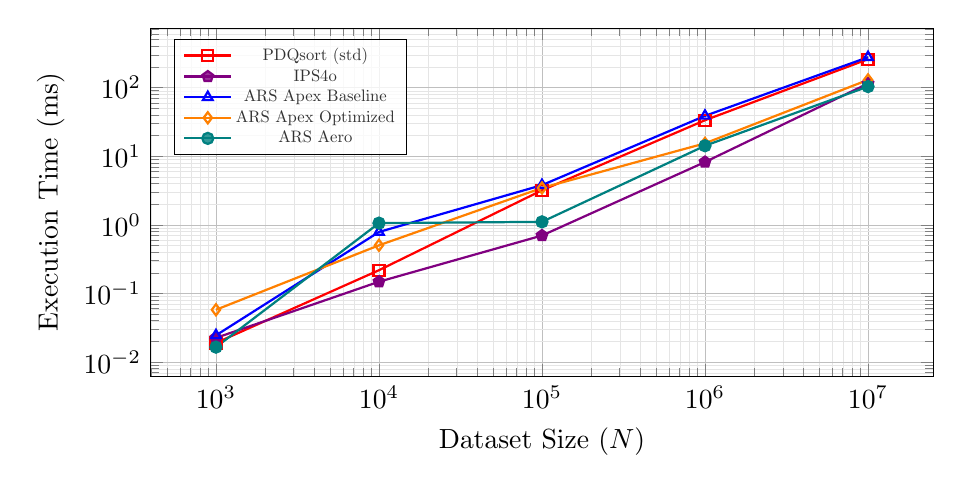
\begin{tikzpicture}
\begin{axis}[
 width=0.95\linewidth, height=6cm,
 xmode=log, ymode=log,
 xlabel={Dataset Size ($N$)},
 ylabel={Execution Time (ms)},
 legend pos=north west,
 grid=both,
 major grid style={line width=.2pt,draw=gray!50},
 minor grid style={line width=.1pt,draw=gray!20},
 legend style={nodes={scale=0.6, transform shape}, fill=white, fill opacity=0.8, draw opacity=1}
]
\addplot[color=red, mark=square, thick] coordinates {
 (1000,0.0190) (10000,0.2180) (100000,3.1853) (1000000,33.4045) (10000000,259.0647)
}; \addlegendentry{PDQsort (std)}
\addplot[color=violet, mark=pentagon*, thick] coordinates {
 (1000,0.0225) (10000,0.1482) (100000,0.6979) (1000000,8.2134) (10000000,114.4291)
}; \addlegendentry{IPS4o}
\addplot[color=blue, mark=triangle, thick] coordinates {
 (1000,0.0245) (10000,0.7865) (100000,3.7867) (1000000,38.6870) (10000000,276.6839)
}; \addlegendentry{ARS Apex Baseline}
\addplot[color=orange, mark=diamond, thick] coordinates {
 (1000,0.0578) (10000,0.5028) (100000,3.4457) (1000000,15.3963) (10000000,129.4175)
}; \addlegendentry{ARS Apex Optimized}
\addplot[color=teal, mark=*, thick] coordinates {
 (1000,0.0165) (10000,1.0580) (100000,1.1045) (1000000,14.1855) (10000000,103.3404)
}; \addlegendentry{ARS Aero}
\end{axis}
\end{tikzpicture}
\caption{Evolution of ARS execution time against PDQsort (i64 Random).}
\label{fig:evolution}
\end{figure}
